% PROJECT: <ETD> Electronic Thesis and Dissertation Initiative
%   TITLE: LaTeX report template for ETDs in LaTeX
%  AUTHOR: Neill Kipp, nkipp@vt.edu
%     URL: http://etd.vt.edu/latex/
% SAVE AS: etd.tex
% REVISED: September 6, 1997 [GMc 8/30/10]

% Instructions: Remove the data from this document and replace it with your own,
% keeping the style and formatting information intact.  More instructions
% appear on the Web site listed above.

%\documentclass[12pt,dvips]{report}
\documentclass[12pt]{report}
\setlength{\textwidth}{6.5in}
\setlength{\textheight}{8.5in}
\setlength{\evensidemargin}{0in}
\setlength{\oddsidemargin}{0in}
\setlength{\topmargin}{0in}
\setlength{\parindent}{0pt}
\setlength{\parskip}{0.1in}
% Uncomment for double-spaced document.
% \renewcommand{\baselinestretch}{2}
% \usepackage{epsf}

%my packages
%packages I used
\usepackage{verbatim}
\usepackage{latexsym}
\usepackage{amsmath, amsfonts, amssymb}
\usepackage{graphicx}
\usepackage{url}
% stuff copied from Bert's paper
\usepackage{color}
%\newcommand{\todo}[1]{\textcolor{red}{\textbf{todo: #1}}}
\newcommand{\then}{\Rightarrow}
\newcommand{\softor}{\operatornamewithlimits{\tilde{\vee}}}
\newcommand{\softand}{\operatornamewithlimits{\tilde{\wedge}}}
\newcommand{\softthen}{\operatornamewithlimits{\tilde{\then}}}
\newcommand{\softneg}{\operatornamewithlimits{\tilde{\neg}}}
\def\RVs{\mathbf{X}}
\def\RV{{X}}
\def\rvpt{{\mathbf{x}}}
\def\reals{{\mathbb{R}}}
\def\extReals{{\mathbb{R}^{\infty}}}
\def\potentials{{\phi}}
\def\potential{{\phi}}
\def\prob{{\mathbb{P}}}
\def\density{{f}}
\def\psl{{PSL}}
\def\Cineq{{B}}
\def\Ceq{{A}}
\def\bineq{{b}}
\def\beq{{a}}
\def\domain{{\mathbf{D}}}
\def\kineq{{k_B}}
\def\keq{{k_A}}

\begin{document}
\thispagestyle{empty}
\pagenumbering{roman}

\begin{center}
% TITLE
{\Large 
Automated Vocabulary Creation For Elections
}
\vfill
Aravindan Mahendiran
\vfill
Thesis submitted to the Faculty of the \\
Virginia Polytechnic Institute and State University \\
in partial fulfillment of the requirements for the degree of
\vfill
Master of Science \\
in \\
Computer Science and Applications
\vfill
Naren Ramakrishnan, Chair \\
Cal Ribbens \\
Aditya Prakash
\vfill
December 25, 2013 \\
Blacksburg, Virginia
\vfill
Keywords: Forecasting, Dynamic Query Expansion, Elections, Probabilistic Soft Logic \\
Copyright 2013, Aravindan Mahendiran
\end{center}
\pagebreak
\thispagestyle{empty}

\begin{center}
{\large Automated Vocabulary Creation For Elections}
\vfill
Aravindan Mahendiran
\vfill
(ABSTRACT)
\vfill
\end{center}
Twitter mining over the last few years has garnered a lot of attention from the research community. 
Strong correlations have been shown between Twitter \emph{‘mentions’} and stock markets, book sales and flu outbreaks which is then used for forecasting.
Even though such methodologies are accurate in forecasting the trends to a great extent, their performance is dictated by the domain specific vocabulary is used to track the relevant tweets. 
Such a vocabulary is usually provided by subject matter experts but is not exhaustive.
The language used in Twitter is drastically different from other forms of writing like those in news articles or even web blogs.  
It constantly evolves with time as users adopt popular hashtags to express their opinion.
Thus, the vocabulary used by the forecasting algorithms needs to be dynamic in nature and should capture the rising trends of the domain. 
Otherwise, the prediction algorithms miss out on capturing the some of the most informative documents.
\newline 
We propose a novel unsupervised learning algorithm builds a vocabulary through modeling user preferences by exploiting the explicit and latent structure in such data sets.
We use Probabilistic Soft Logic, a framework for probabilistic reasoning over relational domains, to develop a query expansion algorithm that learns such a dynamic vocabulary for any given domain.  
Using 7 presidential elections from Latin America we show how such a query expansion methodology improves the recall and accuracy of two state of the art election prediction algorithms. 
Through this approach we achieve close to 2x increase in the recall and 15.5\% reduction in the prediction error. 
\pagebreak

% Dedication and Acknowledgments are both optional
\chapter*{Dedication}
\vspace*{\fill}
\begin{center}
\Large\textit{To my awesomest brother, mother and friends}
\end{center}
\vspace{\fill}

\chapter*{Acknowledgments}
\vspace*{\fill}
\Large{First and foremost I would like to thank my advisor Dr.Naren Ramakrishnan. He was a mentor in every sense of the word and played a vital role in kindling my interest for data mining and machine learning.
\newline I would like to thank my colleagues Sathappan Muthiah, Rupinder Paul Khandpur. Without their support and help, I could not have completed my graduate study. 
}
\vspace{\fill}

\tableofcontents
\pagebreak

\listoffigures
\pagebreak

\listoftables
\pagebreak

\pagenumbering{arabic}
\pagestyle{myheadings}

%\doublespacing


\chapter{Introduction}
\markright{Aravindan Mahendiran \hfill Chapter 1. Introduction \hfill}

\section{Motivation}


\section{Related Work}
The last decade has seen a massive explosion of on-line data in all forms be it news articles,blogs or social media like twitter or Facebook. Twitter alone which came into being only in 2006 has now grown so big \footnote{As of May 7,2013 twitter has 555m active registered users with 135000 new users signing up everyday and approximately 1 billion tweets created every 5 days} that it has come to be looked at as a treasure trove of mine-able data. With free API's to collect this data, the easy access to large volumes of data alone has piqued the interest of research scientists in this domain. Researchers have studied various real world time series and have shown strong correlations of on-line chatter to book sales, box office earnings and even stock prices.~\cite{gruhl2005predictive,asur2010predicting,bollen2011twitter}. Not only did they find correlations but they also were able to "with reasonable accuracy" make forecasts about future trends too. The more curious research is whether such on-line chatter be used to model the social, economic and political landscape of a country. Bollen et al. ~\cite{bollen2011modeling} used a version of the well-established psychometric instrument- Profile of Mood States(POMS) to model the mood of twitter traffic and correlate it to a number of social and economic events that occurred during the same time line. The results from this research instigated more researchers to study and quantify the political sentiment through social media and if possible even forecast election results.
\paragraph{}
We divide the rest of this literature review into four parts. First, we look at a selection of methodologies aimed at predicting elections through volume based approaches. Second, we look at more sophisticated approaches that aim to model the demographics of an election to make informed decisions about such predictions. Then, we shall summarize a quite prevalent pessimistic view on such methodologies' and data sets' capability to predict elections.
\subsection{Volume based approaches}
In one of the most cited papers in this space, Tumasjan et al. ~\cite{tumasjan2010predicting} claim that \emph{ "The mere number of tweets reflect voter preferences and comes close to  traditional polls.."} while predicting  the 2010 German federal election by counting candidate mentions on twitter. They go on to strongly conclude that twitter can indeed be a valid indicator of political opinion. This was followed by ~\cite{o2010tweets,saez2011total,bermingham2011using,demartini2011analyzing} all of which use a volume based approach combined with sentiment analysis. Both ~\cite{o2010tweets,bermingham2011using} fit a regression model to opinion polls with volume share and sentiment as independent variables and conclude that sentiment is a weak predictor compared to share of volume. In general the experiments described in these publications count the occurrence of certain hand filtered keywords in the "twittersphere" and classify such tweets as positive or negative using a classifier trained on human annotated lexicons. A little advanced sentiment classifiers also provide the likelihood that given sample of text belongs to a empirically defined psychological and structural categories like anxiety, anger,sadness etc. 
\subsection{Profile Modeling}
% modelling papers come here
The more sophisticated approach adapted in ~\cite{livne2011party,conover2011predicting,diaz2012taking} is to model the candidates or voters in the elections rather than compute the aggregated sentiment of the mass.  Conover et al. build a SVM trained on manually labled tweets and hash-tags obtained through co-occurrence discovery classify users into 'left' and 'right' aligned. Through latent semantic analysis they claim to have identified the hidden structure in the data that is strongly associated with the political affiliations. Using this information and how political information diffuses in a network, they show  an accuracy of 95\%  in predicting the political alignment of twitter users. Livne et al. in ~\cite{livne2011party} analyse the twitter profiles of candidates from the 2010 mid term elections in the U.S. They identify topics specific to groups of candidates, split according to their known political orientations and use the features obtained as inputs to a regression model to predict the elections. In a similar technique Diaz-Aviles in ~\cite{diaz2012taking} model the candidates by building a emotional vector for each candidate contesting in the elections by using the mentions of that candidate and sentiments associated with each mention learnt using the NRC EmotionLexicon(EmoLex). They use these profiles learnt to predict the rise and fall of a candidate's popularity. In another research, Mustafaraj et al. ~\cite{mustafaraj2011vocal} model the distribution of political content among users in twitter. They claim that there is a spectrum of users in twitter, they dub them as "vocal minority" and "silent majority" and observe these two groups engage in different ways in social media. They show that, the vocal minority aim to broaden the impact of tweets by re-tweeting and linking to outside links whereas the silent majority who tweet significantly lesser are more inclined to share their personal view points. Though they do not make any predictions about elections, they make very valid observations such as \emph{"Because of this differences between content generated by different groups , one should be aware of aggregating data and building models upon them, without verifying the underlying model that has generated the data."}.
% ~\cite{sobkowicz2012opinion}....but try and understand what to summarize from the paper...paper in itself is very abstract.
% ~\cite{huang2012social,kimmig2012short} and write up about how this is the closely related to ur methodologies.
% ask Naren if modeling in PSL should be lit. review or part of methodology.
\subsection{Flaws in current state of the art and recommendations for the future}
Of late there has been a lot of studies showing how such models that predict elections using social media feeds are flawed ~\cite{metaxas2011not,gayo2012wanted,gayo2011don,gayo2011limits}. These publications not only list the obvious issues in using twitter as a input to predict elections but also detail recommendations on how to make such methodologies fool proof. Daniel Gayo-Avello surveys almost all the state of the art approaches in predicting elections in his paper ~\cite{gayo2012wanted} most of which is detailed above. According to him post-hoc analysis of elections in retrospect must not count as valid predictions and also states that researchers do not report negative results leading to what is called the \emph{file drawer} effect. His major points of argument against such models are:
\begin{itemize}
\item
The models are tailor made to fit a particular election and that they need to be generic enough and must be able reproduce similar results when run on other elections. In particular Metaxas et al in ~\cite{metaxas2011not} state that any method claiming predictive power on the basis of Twitter data should be a clearly defined algorithm and should be "explainable" i.e., black box approaches should be avoided.
\item
There is no predefined notion of "vote" that has been used to predict the elections. Most of the models aim to predict elections merely based on volume of tweets related to a candidate and sentimental analysis of such tweets.
\item
Biases in twitter are ignored. Twitter is not a representative sample of the electorate demographic as that not every age gender or social group is represented. He also notes that since people tweet on a voluntary basis the data produced is only by those who are politically active. Another important point of contention relating to bias is the credibility of tweets, whether the tweets are rumors, campaign propaganda or contain misleading information just to maliciously attack candidate's popularity on-line.
\item
Since in 2008 and 2010 , 91.6\% and 84\% of elections were won by the the incumbent candidate respectively, Gayo-Avello argues that incumbency should be the baseline rather than just chance.He also notes that most of the methodologies are only slightly better than chance.
\item
He goes on to argue sentiment analysis and classifiers, though a highly researched subject in NLP, do not perform any better than random classifiers and that these sentiment analysis techniques should be specifically built to handle the political corpus to detect humour and sarcasm which in his opinion would play a major role.
\item
Lastly in ~\cite{gayo2011don} Gayo-Avello akin to ~\cite{mustafaraj2011vocal} states that abstaining from tweeting about politics can play even more important role than the ones mentioning the candidates and hence researches should also model this lack of chatter about a particular candidate or political party.
\end{itemize}
\section{Contributions}
In this work, we attempt to address the following objectives,
\begin{itemize}
\item
Design and implement a new dynamic query expansion algorithm using Probabilistic soft logic.
\item
Compare and contrast the vocabulary obtained by PSL to baseline DQE.
\item
Build state of the art models for election predictions.
\item
Show how using the distilled vocabulary from the Dynamic Query Expansion exercise improves the accuracy of prediction algorithms.
\end{itemize}

\section{Document Overview}
The rest of the document is structured as follows.
\chapter{Dynamic Query Expansion}
\markright{Aravindan Mahendiran \hfill Chapter 2. Dynamic Query Expansion\hfill}
\section{Query Expansion}
In most document corpora, a single concept can be referred using multiple terms.
In information retrieval (IR) this is called \emph{synonymy} and has a huge impact on the recall of documents pertaining to the concept.
Researchers address this problem by creating as exhaustive a query as possible. 
But when exploring the Twitter corpora it becomes almost impossible to hand craft such a expansive query as the meme and hash-tag adaptations are not known a priori. 
\newline
To address this issue IR experts use \emph{query expansion} or reinforcement learning.
These are iterative algorithms that are initialized with a small set of query terms. 
When the documents matching the query terms are returned, after basic  processing such as tokenization, stop-word removal and stemming a richer vocabulary is obtained by ranking the terms in these documents by their frequency counts.
The top words from this list is then used to query the documents again. 
This process goes on until no new terms are added to the vocabulary. 
We design and implement such an pipeline using Probabilistic Soft Logic to build our vocabulary for a given election. 
We first review the PSL framework before proceeding to detail our methodology.
\section{Probabilistic Soft Logic}
Probabilistic Soft Logic ~\cite{kimmig2012short} is a framework for collective probabilistic reasoning on relational domains.
PSL models have been developed in various domains, including collective classification ~\cite{broecheler2010computing}, ontology alignment ~\cite{brocheler2012probabilistic}, personalized medicine ~\cite{bach2010decision}, opinion diffusion ~\cite{bach2012scaling} , trust in social networks ~\cite{huang2012probabilistic}, and graph summarization ~\cite{memory2012graph}.
PSL represents the domain of interest as logical atoms.
It uses first order logic rules to capture the dependency structure of the domain, based on which it builds a joint probabilistic model over all atoms.
Instead of hard truth values of $0$ (false) and $1$ (true), PSL uses soft truth values relaxing the truth values to the interval $[0,1]$.
The logical connectives are adapted accordingly.
This makes it easy to incorporate similarity or distance functions.
\newline
User defined \emph{predicates} are used to encode the relationships and attributes and \emph{rules} capture the  dependencies and constraints.
Each rule's antecedent is a conjunction of atoms and its consequent is a dis-junction. 
The rules can also labeled with non negative weights which are used during the inference process. 
The set of predicates and weighted rules thus make up a PSL program where known truth values of ground atoms are set from observed data and unknown truth values for the remaining atoms are learned using the PSL inference mechanism.
\newline
Given a set of atoms 
$\ell = \{\ell_1,\ldots,\ell_n\}$,
an interpretation defined as 
$I : \ell \rightarrow [0,1]^n$
is a mapping from atoms to soft truth values.
PSL defines a probability distribution over all such interpretations such that those that satisfy more ground rules are more probable.
\emph{Lukasiewicz t-norm} and its corresponding co-norm are used for defining relaxations of the logical AND and OR respectively to determine the degree to which a ground rule is satisfied.
Given an interpretation $\mathit{I}$, PSL defines the formulas for the relaxation of the logical conjunction ($\wedge$), dis-junction ($\vee$), and negation ($\neg$) as follows:

\begin{align*}
\ell_1 \softand \ell_2 &= \max\{0, I(\ell_1) + I(\ell_2) - 1\},\\
\ell_1 \softor \ell_2 &= \min\{I(\ell_1) + I(\ell_2), 1\},\\
\softneg l_1 &= 1 - I(\ell_1),
\end{align*}  
where we use \textasciitilde to indicate the relaxation of the Boolean domain.
The interpretation $\mathit{I}$ determines whether the rules is satisfied, if not, the \emph{distance to satisfaction}.
A rule $\mathit{r} \equiv \mathit{r_{body}} \rightarrow \mathit{r_{head}} $  is satisfied if and only if the truth value of head is atleast that of the body. The rule's distance to satisfaction measures the degree to which this condition is violated.
 \newline
\begin{center} 
 $\mathit{d_r}(\mathit{I}) =$ max\{0,$\mathit{I(r_{body}} - \mathit{I(r_{head}}$\}
 \end{center}

PSL then induces a probability distribution over possible interpretations $\mathit{I}$ over the given set of ground atoms $\mathit{l} $ in the domain. 
If $\mathit{R}$ is the set of all ground rules that are instances of a rule from the system and uses only the atoms in  $\mathit{I}$ then,
the probability density function $\mathit{f}$ over $\mathit{I}$ is defined as
\begin{equation}
\label{eq:contimn1}
    f (I) = \frac{1}{Z} \text{exp}[-\sum_{r\in R} \lambda_r (d_r(I))^p]
\end{equation}
\begin{equation}
\label{eq:contimn2}
	Z = \int_{I} \text{exp} [ -\sum_{r\in R} \lambda_r (d_r(I))^p ]
\end{equation}
where~$\lambda_r$ is the weight of the rule~$r$, $Z$ is the continuous version of the normalization constant used in discrete Markov random fields, and ~$p \in \{1, 2\}$ provides a choice between two different loss functions, linear and quadratic.
The values of the atoms can be further restricted by providing linear equality and inequality constraints allowing one to encode functional constraints from the domain.
\paragraph{}
PSL provides for two kinds of inferences (a)most probable explanation and (b)calculation of the marginal distributions. 
In the MPE inference given a partial interpretation with grounded atoms based on observed evidence, the PSL program infers the truth values for the unobserved atoms satisfying the most likely interpretation. 
In the second setting, given ground truth data for all atoms we can learn the weights for the rules in our PSL program.
In our work we leverage the MPE inference.
\section{Dynamic Query Expansion using PSL}
In ~\cite{huang2012social}, we used PSL to model user affiliations within groups. 
Specifically we built a PSL program for a  social network where we have a set of users, their posts, messages to other users and the various groups we want to model. 
The rules we defined captured the dynamics of group affiliations through the various interactions.
Through the MPE inference we classified users into different groups based on their hash-tag usage and their interactions with other users.
\paragraph{}
In this paper we extend our earlier work to achieve what we call dynamic query expansion through PSL. 
Similar to the query expansion methodology described earlier we start with an initial set of hash-tags which we believe are indicative of the affinity of a particular user to a candidate contesting in the election.
We refer to these hash-tags as seed words.
Instead of a single inference, we iteratively perform the inference over successive time windows such that the inference from window $w_t$ is used as a prior to window $w_{t+1}$ and the inference from that is used for window $w_{t+2}$ and so on.
\begin{figure*}[Ht]
	\centering
	%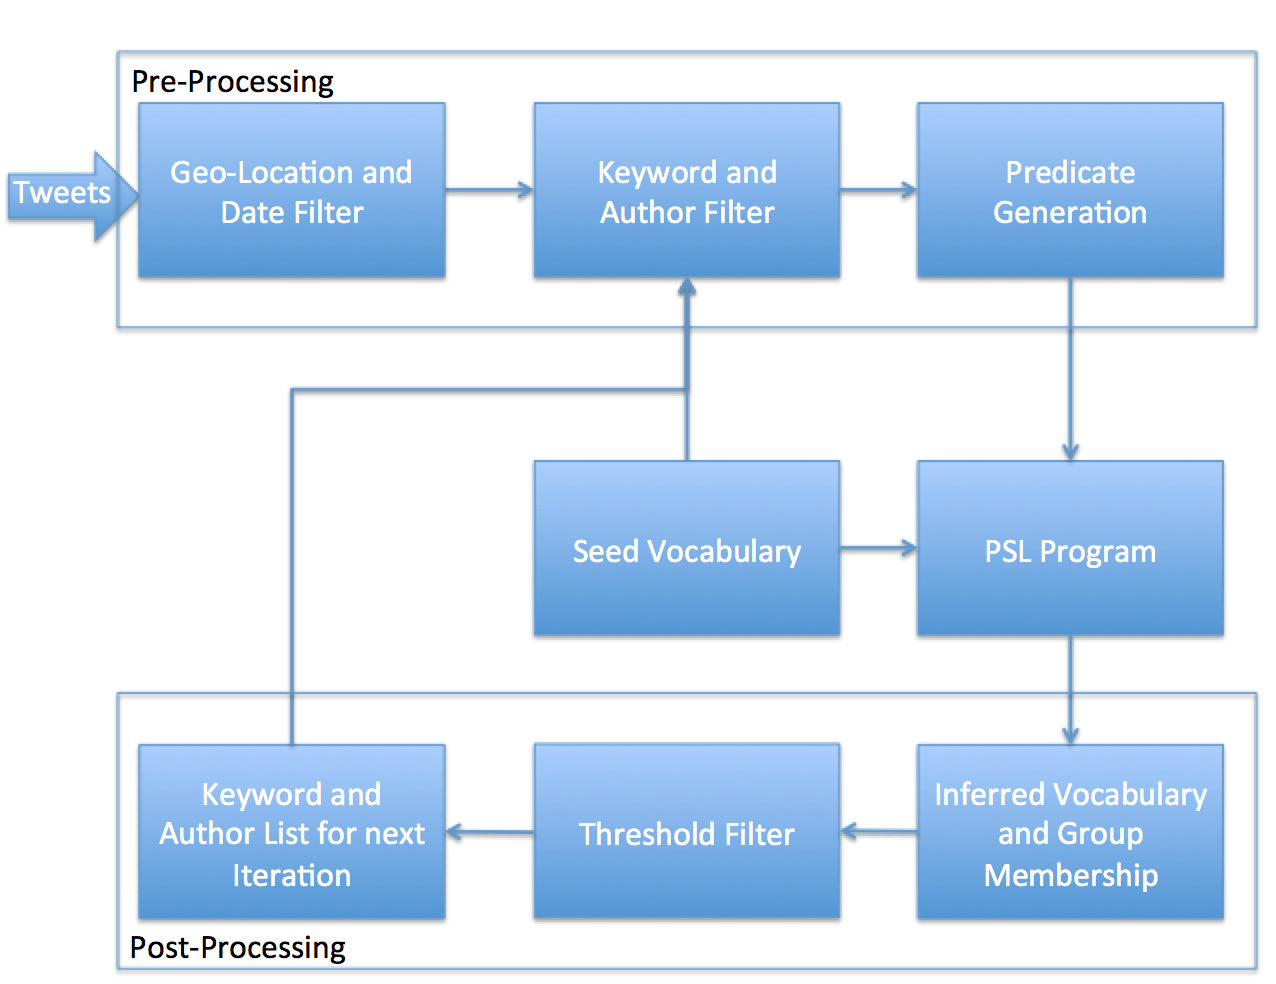
\includegraphics[scale=0.50]{support_files/flowChart.png}
	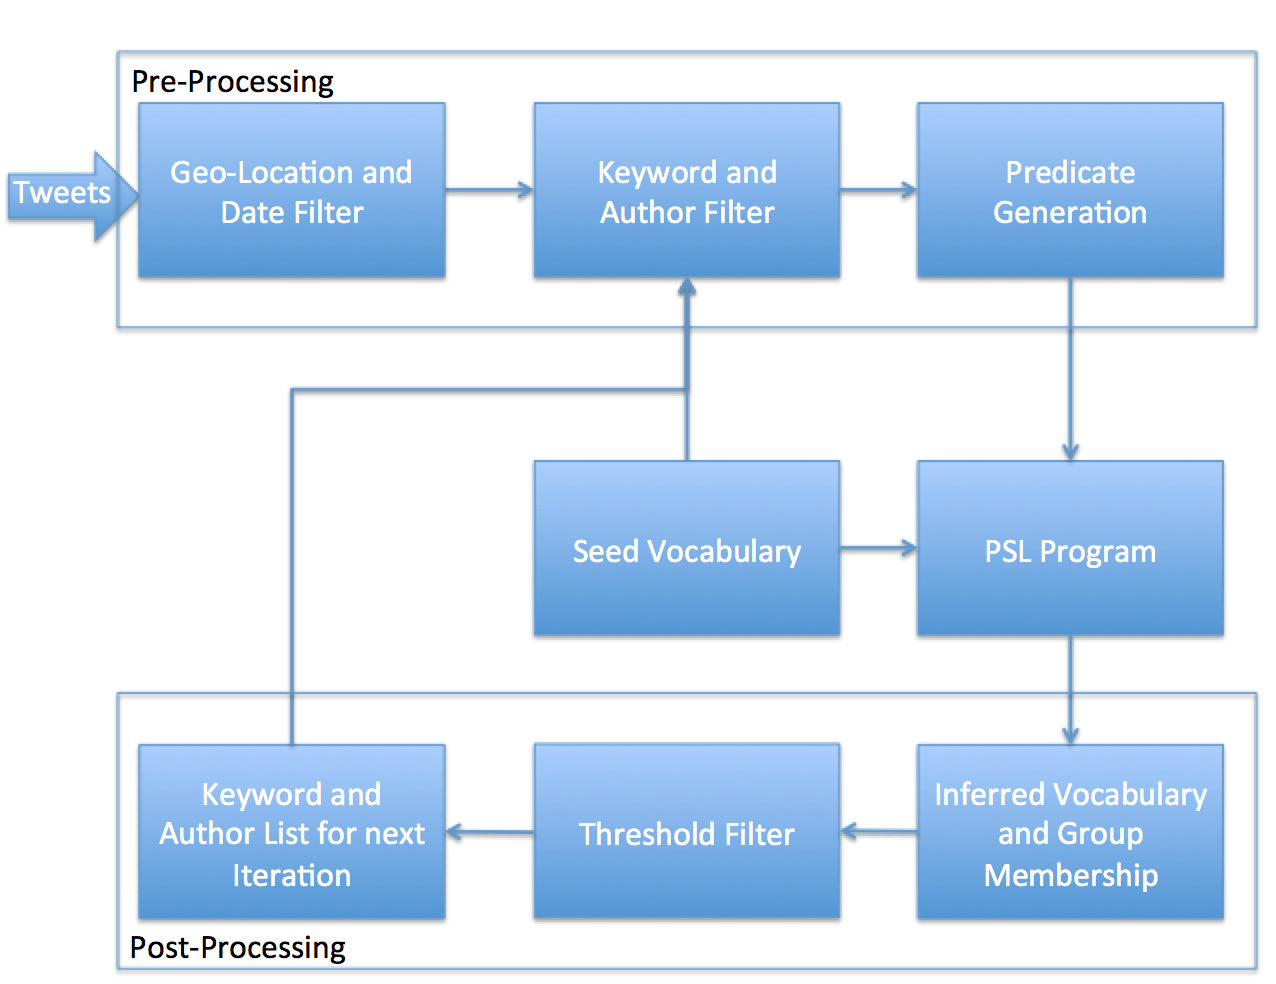
\includegraphics[height=0.5\textheight, width=1.0\textwidth]{support_files/flowChart.png}
	\caption{Design of the query expansion pipeline.}
	\label{fig:flowchart}
\end{figure*}
\paragraph{}
Figure\ref{fig:flowchart} illustrates the design of the iterative algorithm for dynamic query expansion.
The initial pre-processing starts with the tweet input stream which is filtered by the date range specified by the window size. 
For each election, tweets from a month leading up to the election were used.
After extensive analysis it was determined that the most optimal window size was 3 days. 
Smaller window sizes resulted in sub-optimal inferences as there were not enough data points feeding into the PSL stage.
Larger window sizes lead to memory issues as the PSL optimization has a time complexity of  $O(n^{3.5})$ where $n$ is the number of relevant rule groundings, i.e., those with non-zero distance to satisfaction. 
The tweets passing the date filter are then geo-coded using a geo-location algorithm that infers the location of a tweet. 
This ensures that only tweets originating from the country of interest are used.
The geo-location algorithm tags the tweets with a location by looking at the GPS coordinates of the tweet if available or landmarks and locations mentioned in the tweet or author's profile. 
For tweets that do not have either of these information it uses a label propagation algorithm to infer the author's location through his/her network.
\newline
The geo-tagged tweets are then tracked for the presence of a hash-tag from the vocabulary for that particular iteration.
In addition to filtering tweets using the vocabulary the authors whose affiliations are already inferred by the system are also used as a filtering criteria.
The tweets are then converted into PSL predicates and fed into the inference process.
The PSL program infers the hash-tags and tweeters that are mostly associated with a particular candidate. 
Each author and hash-tag's association with a candidate is measured using the truth value of the predicate grounding.
In the post-processing step, these truth values are filtered by a threshold value to identify the hash-tags and authors strongly associated to a candidate.
These hash-tags become a part of the vocabulary of the candidate and along with the users identified are used as a filter criterion for the next iteration.
This iterative process proceeds until the day before the election when we obtain the final vocabulary which are strongly associated with a candidate.
\paragraph{}
Within the PSL program we define predicates to encode the network. 
The predicates $Tweeted(U,T)$ and $Contains(T,W)$  capture the fact that a user $U$ tweeted a tweet $T$ and tweet $T$ contains hash-tag $W$ respectively. 
Similarly, the belief that a user $U$ or hash-tag $W$ is affiliated/associated to the group $G$ is encoded as $Is\_Member(U,G)$ and $Belongs(W,G)$ respectively.
In order to capture the temporal connectivity between the iterations, in addition to the initiating the inference process with the rule
\begin{align*}
Seed\_Word(W,G) \Rightarrow Belongs(W,G)
\end{align*}
we define additional rules such as
\begin{align*}
Was\_Member(A,G) \Rightarrow Is\_Memeber(A,G)
\end{align*}
\begin{align*}
Belonged(W,G) \Rightarrow Belongs(W,G)
\end{align*}
where the predicates $Was\_Member$ and $Belonged$ are inferences from the previous time window and are loaded in as  priors for the current iteration.
These rules are weighted slightly lower than the recursive rules below so that the system overcomes the bias it had learned in light of new more convincing evidence.
This way hash-tags that are more indicative of a user's affiliation are assigned stronger truth values or weights for every successive iteration and the weights hash-tags that aren't are reduced.
The same reasoning applies to the user-candidate affiliations(memberships) too.
Below we outline the recursive PSL rules that grows the hash-tag preferences and the user affiliations. 
\begin{align*}
\begin{split}
Tweeted(A,T) 
	\softand Contains(T,W)
	\softand Belongs(W,G) \\ 
	\softand Positive(T)
	\Rightarrow Is\_Member(A,G)
\end{split}
\end{align*}

\begin{align*}
\begin{split}
Tweeted(A,T)
	 \softand Contains(T,W)
	\softand Belongs(W,G)\\
	 \softand Negative(T)
	\Rightarrow \sim Is\_Member(A,G)
\end{split}
\end{align*}

\begin{align*}
\begin{split}
Is\_Member(A,G)
	 \softand Tweeted(A,T)
	\softand Contains(T,W)\\
	 \softand Positive(T) 
	\Rightarrow Belongs(W,G)
\end{split}
\end{align*}

\begin{align*}
\begin{split}
Is\_Member(A,G) 
	\softand Tweeted(A,T)
	\softand Contains(T,W)\\
	\softand Negative(T)
	\Rightarrow \sim Belongs(W,G)
\end{split}
\end{align*}
Here $Positive$ and $Negative$ are predicates whose truth values are calculated from the sentiment of the tweet such that the highly positive tweets get a truth value closer to $1.0$ for the predicate $Positive$ and highly negative tweets are assigned a truth value of $1.0$ for the predicate $Negative$. 
Since PSL works under the close world assumption, we do not need to specify the groundings that are false i.e., positive tweets are not assigned $0.0$ for the predicate $Negative$ and vice-versa.
\begin{figure*}
	\centering
	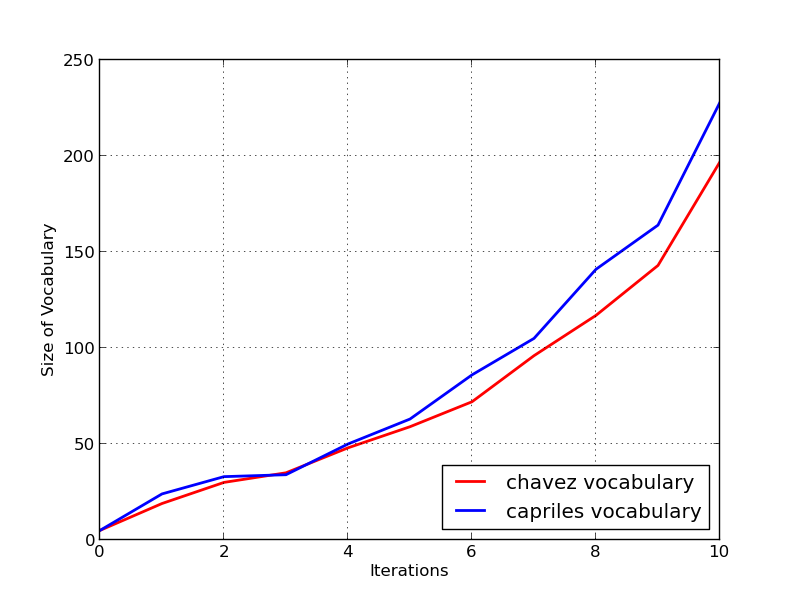
\includegraphics[scale=0.50]{support_files/WordGrowth.png}
	\caption{Vocabulary growth with each iteration.}
	\label{fig:wordgrowth}
\end{figure*}
For tweets that do not have a positive or negative orientation we assign a truth value of $0.5$ for both the $Positive$ and $Negative$ predicates.\\
The last two rules defined below encode the assumption that when two hash-tags co-occur and one is a name of a candidate then the other hash-tag is bound to be about the candidate too.
\begin{align*}
\begin{split}
Contains(T,W1)
 \softand Contains(T,W2)
  \softand Seed\_Word(W1,G)\\ 
  \softand Positive(T)
	\Rightarrow Belongs(W2,G)
\end{split}
\end{align*}

\begin{align*}
\begin{split}
Contains(T,W1) 
	\softand Contains(T,W2)
	\softand Seed\_Word(W1,G)\\ 
	\softand Negative(T)
	\Rightarrow \sim Belongs(W2,G)
\end{split}
\end{align*}
Once all the tweets are loaded into the PSL program as predicates, we start the inference process by closing all the predicates except $Is\_Member$ and $Belongs$. 
This way, only their truth values are inferred.
\section{Results}
\begin{figure*}
	\centering
	\subfloat[Day 0]
	{
		
\includegraphics[width=0.5\textwidth, height=0.20\textheight]{support_files/caprilesWordCloud1.png}
		\label{fig:wordCloud1}
	} 
	\subfloat[Day 6]
	{
		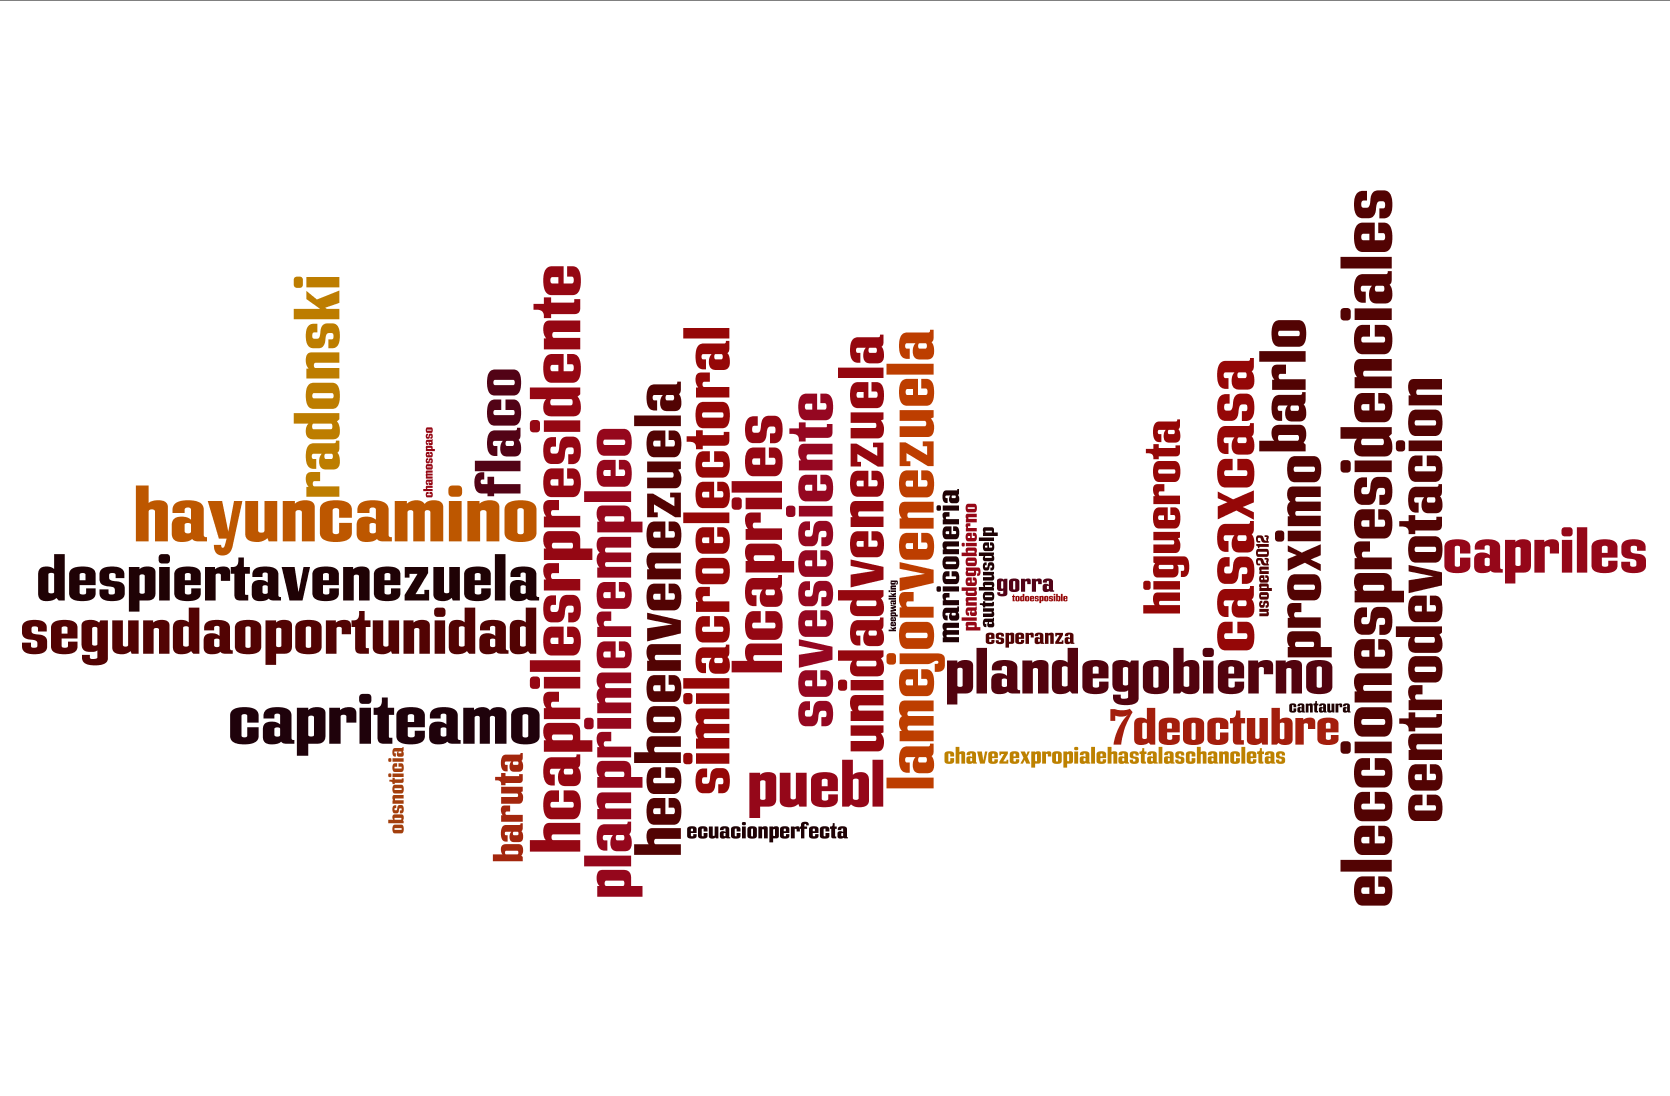
\includegraphics[width=0.5\textwidth, height=0.20\textheight]{support_files/caprilesWordCloud2.png}
		\label{fig:wordCloud2}
	} \\
	\noindent 
	\subfloat[Day 15]
	{
		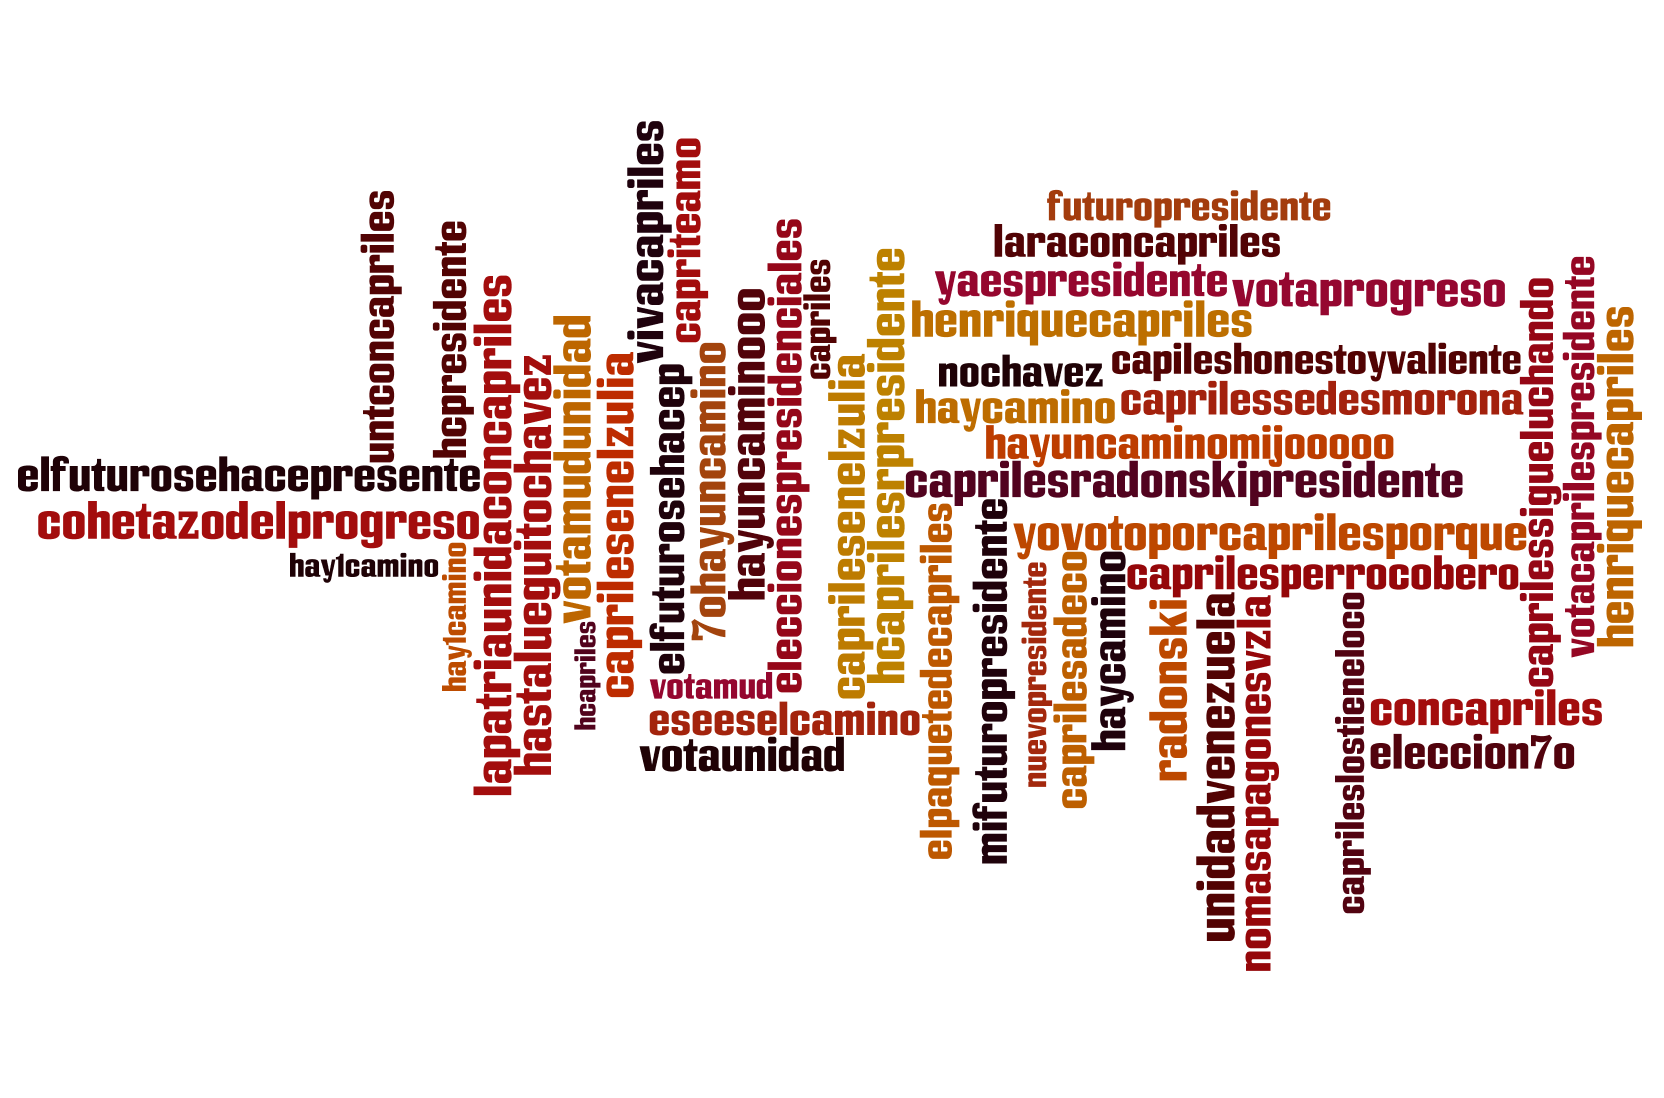
\includegraphics[width=0.5\textwidth, height=0.20\textheight]{support_files/caprilesWordCloud3.png}
		\label{fig:wordCloud3}
	}
	\subfloat[Day 30]
	{
		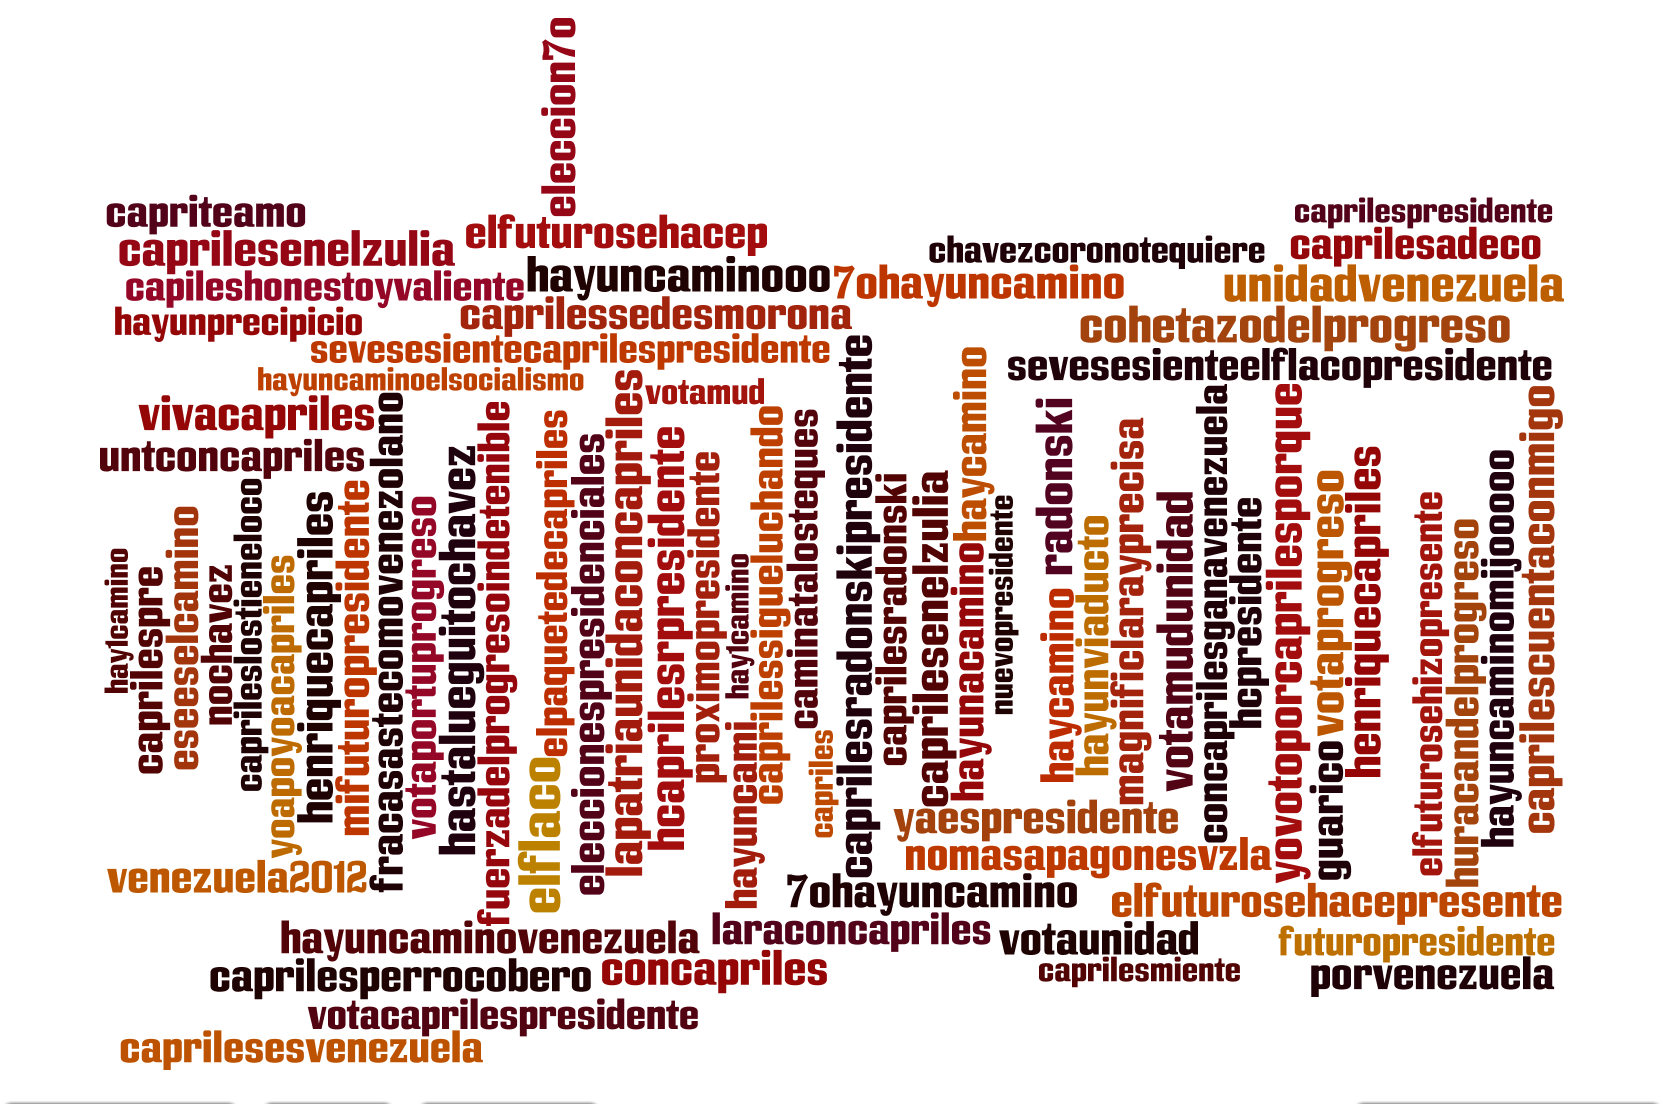
\includegraphics[width=0.5\textwidth, height=0.20\textheight]{support_files/caprilesWordCloud4.png}
		\label{fig:wordCloud4}
	}
	\caption{Evolution of hash-tags for Henrique Capriles} 
	\label{fig:wordCloud}
\end{figure*}

Figure\ref{fig:wordgrowth} shows  how the vocabulary grows with each iteration for the two candidates who contested the Venezuelan presidential election on October 7th 2012.\\
Figure\ref{fig:wordCloud} shows how the hash-tags for Henrique Capriles evolved during the month leading up to the election.
Initially in Figure\ref{fig:wordCloud1} the system starts with only a few hand picked hash-tags that constitute the seed vocabulary. 
After a few iterations Figure\ref{fig:wordCloud2} shows how the vocabulary has grown.
However, not all the words identified until now remain in the final vocabulary as the system drops certain words in successive iterations.
At the same time it is also noticed that hash-tags like "capriles" and "hayuncamino" which are very strongly associated with Capriles consistently remain as the top ranked hash-tags even after ten iterations(Figure\ref{fig:wordCloud4}). 
It is also interesting to note that the algorithm identified hash-tags like "nochavez"(Figure\ref{fig:wordCloud3}) and attributed it rightly to Hugo Chavez's primary contender- Capriles. \\
\begin{figure*}[Ht]
	\centering
	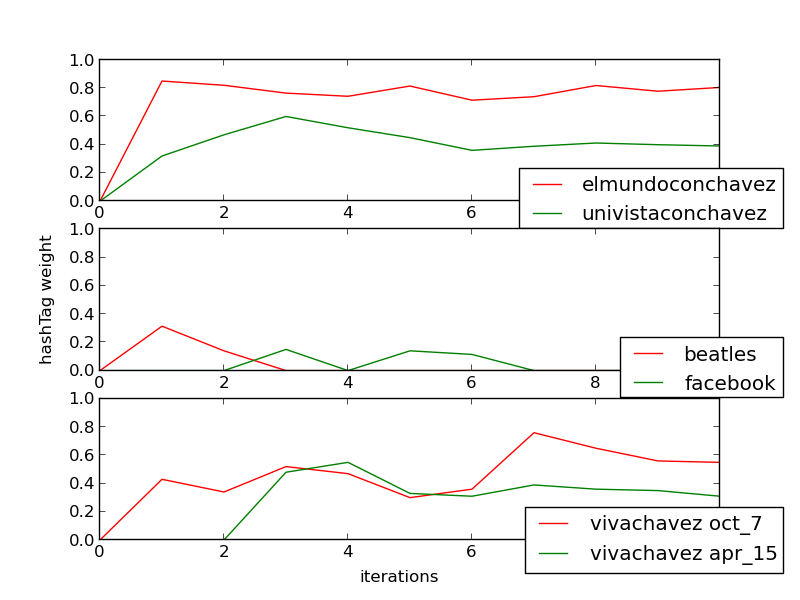
\includegraphics[scale=0.65]{support_files/hashTagTimeSeries.png}
	\caption{Time series comparison for different hash-tags identified for Hugo Chavez.}
	%The first plot shows "univistaconchavez" and "elmundocochavez". The second plot shows "Beatles" and "Facebook". The third plot shows "vivachavez" from two different elections conducted on 15th April 2013 and 7th October 2012.
	\label{fig:timeSeries}
\end{figure*}
In figure \ref{fig:timeSeries}, the first plot elucidates how hash-tags like \emph{"elmnduconchavez"} and \emph{"univistaconchavez"} remain highly associated with Hugo Chavez for the October 7th Presidential election. 
These hash-tags remain indicative of a user's affiliation throughout the month leading up to the election.
Meanwhile hash-tags such as \emph{"beatles"} and \emph{"facebook"} ( in second plot) show spikes in their time series primarily because users affiliated with Chavez used them during that time window. 
But as iterative process continues the system drops these non-informative words.
The third plot presents another interesting observation 
The hash-tag \emph{"vivachavez"} is part of both the Venezuelan elections despite the fact that Hugo Chavez did not contest the second election on April 15th 2013. 
It is picked up as a phrase commonly used by supporters of Nicholas Maduro whose election campaign was strategized around the death of Hugo Chavez to garner sympathy and mobilize support.
Similarly variations of the hash-tags \emph{"hayuncamino"} and \emph{"unidadvenuzela"} was returned for Henrique Capriles for both these elections.
\chapter{Prediction Models}
\markright{Aravindan Mahendiran \hfill Chapter 3. Prediction Models \hfill}
In this section we review two prediction models we adapted from current literature to test our hypothesis. 
The first one is a naive model that forecasts elections based on the counts of mentions of a candidate.
We dub this as  \emph{"unique visitor model"} and is adapted from \cite{saez2011total} and \cite{tumasjan2010predicting}.
The second model uses a regression fit to regress from tweet features to opinion polls and then predicts election. 
This we dub as the \emph{"regression model"} and is adapted from \cite{bermingham2011using} and \cite{o2010tweets}.
\section{Unique Visitor Model}
Without any loss of generality, it can be assumed that large parties that are more popular will have a larger social media foot print than smaller and less popular parties. 
This model takes advantage of this assumption and predicts elections by calculating the relative popularity of candidates contesting the election.
We first define a vocabulary for each candidate. 
This vocabulary is crafted by hand and includes the candidate's names and aliases, the name and acronyms for his/her political party and the official Twitter handle of the candidate and is same as the seed vocabulary that was used to initialize the PSL pipeline.
For the given time period, the tweets from the country in question are tracked for the occurrence of the terms in the vocabulary.
We then build a time series of sentiment and Klout scores from the tweets returned.
Klout score is a value provided by Klout.com that quantifies the impact each user has on social media. 
We use the sentiment scores provided as a part of the meta-data of the tweet. 
%The sentiment scores typically fall in the range of $[-15,15]$ and is provided by Lexalytics - a pioneer in linguistic processing.
Once a time series of the Klout and sentiment scores are built, we calculate the absolute popularity of a candidate $C_d$ as:
\begin{equation}
{C_d} = \sum_i K_i * UCS_{id}
\end{equation}
where $K_i$ is the Klout score for user $i$, and $UCS_{id}$ is User Candidate Score, the average of sentiment scores for all tweets from user $i$ about candidate $d$.
We then normalize the popularity scores across all candidates so that they sum to $1$.
This gives us the relative popularity of each candidate $P_d$ using which we predict the elections.
\begin{equation}
{P_d} = \sum_i \frac{C_d}{C_i}
\end{equation}
From the above equations, it is noticeable that each user contributes only once to the popularity score of a candidate.
This was preferred to merely counting the mentions of a candidate since we wanted to remove the bias of bot generated tweets from election campaigns that boosted the number of times a candidate is mentioned on Twitter.
\section{Regression Model}
In this model, in addition to Twitter data, we leverage the opinion polls available for the elections to make our predictions.
Like the earlier model we track the tweets that contain a word from the vocabulary defined for each candidate.
We then define a linear regression fit that uses the opinion polls as dependent variable and features generated from these tweets as independent variable.
We use a total of 6 features based on Klout scores, number of unique users, total number of mentions, sentiment and incumbency.
We normalize each of these features across all candidates to get the relative share of the volume. 
For example for the we define share of positive mentions($SoPM$)  as: 
\begin{equation}
SoPM(x) = \frac{\#PositiveMentions(x)}{\sum_i \#PositiveMentions(i)} 
\end{equation}
and share of negative users($SoNU$) as:
\begin{equation}
SoNU(x) = \frac{\sum_j K_j}{\sum_i \sum_j K_j}
\end{equation}
where $K_j$ is the Klout score of user $j$ who tweeted negatively about a candidate.
Similarly we define share of sentiment ($SoS$) as the sum of all sentiment scores normalized across all candidates. 
We use a binary variable for incumbency. 
We then build a time-line of opinion polls. 
For each of the polling dates we calculate these features by using tweets created during the 10 day window leading up to the polling date.
When we have more than one polling house publishing its opinion poll for the same date we take the average of the polls. 
Once we create a feature set for all the polling dates, we fit a simple least square regression as :
\begin{equation}
\begin{split}
Popularity(x) = \alpha_1 * SoPM(x) + \alpha_2 * SoNM(x) \\
						 + \beta_1 * SoPU(x) + \beta_2 * SoNU(x) \\
						 + \gamma * SoS(x) + \delta * Incumbency(x) + \epsilon
\end{split}
\end{equation}
Table\ref{table:coeff} details the coefficients learned for each feature averaged over all the candidates from all the elections.
The values confirm our hypothesis that the number of unique users and sentiment have more predictive power than total number of mentions.
Intuitively it is also seen that the coefficients for share of negative users and negative mentions carry a negative weight.
Another interesting observation is the fact that the incumbency binary variable is not very predictive which is contradictory to the popular opinion.
\begin{table*}
        \centering
        \begin{tabular}{|l|r|}
        \hline
        Feature & Coefficient Value\\
        \hline
        $SoPU$ & 0.4622\\
        $SoNU$ & -0.443\\
        $SoPM$ & 0.1158\\
        $SoNM$ & -0.065\\
        $SoS$ & 0.156\\
        $Incumbency$ & 0.0\\
        \hline
        \end{tabular}
        \caption{Regression coefficients learned for features}
        \label{table:coeff}
\end{table*}
After learning the regression fit, we make a prediction by building such features using the same 10 day window leading up to the prediction date.
\section{Performance}
\begin{table*}
        \centering
        \begin{tabular}{| l | r | r | r |}
        \hline
        Election Type & Number of Elections & Number of Correct Predictions & Accuracy\\
        \hline
        President/Prime Minister & 8 & 8 & 100\%\\
        Governor & 4 & 3 & 75\%\\
        Mayor & 24 & 12 & 50\%\\
        Overall & 36 & 23 & 63.88\%\\
        \hline
        \end{tabular}
        \caption{Track Record of Prediction Algorithms}
        \label{table:trackRecord}
\end{table*}
The Unique Visitor Model and the Regression Model were tested exhaustively on a total of 36 elections from Latin America during 2012 and 2013 ranging from local mayor elections to presidential elections at the country level.
It is important to note that every single election was predicted ahead of time and not in retrospect.
The tweets were purchased from DataSift, an infoveilence service that resells Twitter data.
On an average we collected close to 2 million unique tweets a day from over 21 countries in Latin and South America.
Then these tweets were geo-coded using a geo-location algorithm we developed to obtain tweets from the country of interest.
Only tweets from the locations pertaining to elections were used to make the predictions.
For example, for the Rio De Janeiro Mayor elections only tweets from the city of Rio De Janeiro were used and similarly for state level Governor elections only tweet originating from that particular state was used.
Once the tweets were filtered by location the time series of Klout and sentiment scores were calculated by tracking the tweets for the mentions of candidate.\\
Table\ref{table:trackRecord} below shows the over all performance of the two models. 
It can be noticed that the accuracy drops as the granularity of the elections reduces. 
This is primarily due to the fact that, opinion polls were available only for the country level elections.
Therefore, we could not use the Regression Model for the state or city level elections.
This increased the error as the predictions were generated only from the naive Unique Visitor Model.\\
Also, from the tweets collected it was noticed that there wasn't much chatter on Twitter about these smaller local elections.
This skewed the results as the model tracking the names of the candidates was using tweets that mentioned the candidate's name but wasn't about the candidate contesting in the election but was about some other person having the same name as the candidate.
If the city level elections were ignored as outliers the over all accuracy of the models improves to 91.6\%.

\chapter{Evaluations and Results}
\markright{Aravindan Mahendiran \hfill Chapter 3. Evaluations and Results \hfill}
To evaluvate our hypothesis we test our models on different elections from Latin America.
The tweets are provided by DataSift, an infoveilence service that resells Twitter data.
On an average we collect close to 2 million unique tweets a day from over 21 countries in Latin and South America.
Then these tweets are geo-coded using a geo-location algorithm we developed to obtain tweets from the country of interest.
We then run the two prediction algorithms to get their baseline perfermance.
These two models have been tested extensively on 36 elections from Latin America from 2012-2013 including Presidential, Governor and Mayoral elections. 
Out of these 36 elections, the models predicted 21 of them correctly. 
%The combined track record for the two elections have been detailed in \ref{table:trackRecord}. 
Importantly every single election was predicted ahead of time and not in reterospect.
The models perform poorly on local mayoral elections(12 out of 24 predicted correctly) as there was not much chatter on Twitter about these elections to make sound predictions. 
The regression model was used only for presidential elections as opinion polls were not available for Governor and Mayoral elections.
Hence we use only the presidential elections to evaluavate our vocabulary.
Once we have the baseline score for these models, we then use the same vocabulary to seed our PSL learning algorithm. 
The prediction algorithms are then run again, now by using the expanded vocabulary obtained through the query expansion at each iteration.
%track record table

\begin{table*}[Ht]
	\centering
	\begin{tabular}{| r || r | r | r | r | r | r |}
 	\hline
 	Election & UniVis+Seed & UniVis+PSL & Improv. & Reg+Seed & Reg.+PSL & Improv\\
 	\hline
	Mexico & 0.353 & 0.368 & -4.2\% & 0.123 & 0.07 & 43.09\% \\ 	
 	Venezuela\_Oct7 & 0.069	& 0.077 & -11.59\% & 0.158 & 0.109 & 31.01\&\\
	Ecuador & 0.531 & 0.547 & -3.01\% & 0.263 & 0.244 & 7.22\% \\
	Venezuela\_Apr15 & 0.198 & 0.178 & 10.10\% & 0.142 & 0.112 & 21.126\&\\
	Paraguay & 0.34 & 0.288 & 15.29\% & 0.2 & 0.18 & 10\% \\
	Chile\_Nov17 & 0.56 & 0.42 & 25\% & 0.245 & 0.207 & 15.51\% \\
	Honduras & 0.563 & 0.527 & 6.39\% & 0.293 & 0.184 & 37.20\% \\
	Chile\_Dec17 & 0.096 & 0.061 & 36.45\% & 0.409 & 0.369 & 9.77\% \\
 	\hline
	\end{tabular}
	\vspace{-0.5em}
	\caption{Performance of models with different vocabs measures using Mean Absolute Percentage Error}
	\label{table:improvement}
	\vspace{-0.5em}
\end{table*}	

\begin{table*}[Ht]
	\centering
	\begin{tabular}{| l | l | l | l |}
	\hline
	Election Type & Number of Elections & Number of Correct Predictions & Accuracy\\
	\hline
	President/Prime Minister & 8 & 7 & 87.5\%\\
	Governor & 4 & 3 & 75\%\\
	Mayor & 24 & 12 & 50\%\\
	Overall & 36 & 22 & 61.1\%\\
	\hline
	\end{tabular}
	\vspace{-0.5em}
	\caption{Track Record of Prediction Algorithms}
	\label{table:trackRecord}
	\vspace{-0.5em}
\end{table*}

\begin{figure*}[Ht]
	\centering
	%\captionsetup{font=scriptsize}
	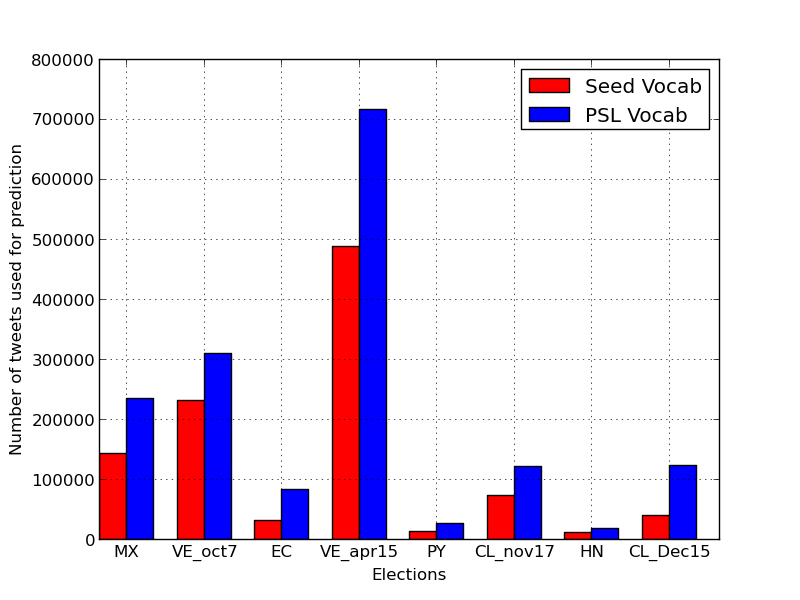
\includegraphics[width=0.7\textwidth, height=0.3\textheight]{support_files/Recall.png}
\vspace{-1em}
	\caption{Recall of seed vocabulary vs PSL vocabulary}
	\label{fig:recall}
	\vspace{-1em}
\end{figure*}
Figure \ref{fig:recall} shows the increase in the number of documents that were used by the algorithm to make a prediciton.
It is noticed when averaged across all the 8 elections we have close to a 2x increase in the number of tweets that were used by these models.
This is a substantial increase in the recall of relevant tweets for the domain.
To further illustrate the fact that the vocabulary used by such algorithms plays a vital role, we compare the performance of the models using the two different vocabularies.
The Mean Absolute Percentage Error (MAPE) was used as a metric to measure the performance of the models. 
To reduce the effect of outliers we track the popularity of only the major candidates and ignore the ones who obtained less than 10\% of the total votes.
Table \ref{table:improvement} shows the performance of each vocabulary in different elections. 
On an average it is seen that the mean absolute percentage error is reduced by 15.58\%.

\chapter{Conclusions and Future Work}
\markright{Aravindan Mahendiran \hfill Chapter 5. Conclusions and Future Work \hfill}
\section{Conclusions}

\label{sec:conclusion}

\section{Future Work}


%%%%%%%%%%%%%%%%%
%
% Include an EPS figure with this command:
%   \epsffile{filename.eps}
%

%%%%%%%%%%%%%%%%
%
% Do tables like this:

%  \begin{table}
%  \caption{The Graduate School wants captions above the tables.}
% \begin{center}
%  \begin{tabular}{ccc}
%  x & 1 & 2 \\ \hline
%  1 & 1 & 2 \\
%  2 & 2 & 4 \\ \hline
%  \end{tabular}
% \end{center}
%  \end{table}

%%%%%%%%%%%%%%%%%%%%%%%%%%%%%%%%

% If you are using BibTeX, uncomment the following:
% \thebibliography
%
% Otherwise, uncomment the following:
% \chapter*{Bibliography}

% \appendix

% In LaTeX, each appendix is a "chapter"
% \chapter{Program Source}

\cleardoublepage
%\phantomsection
\addcontentsline{toc}{chapter}{Bibliography}
\bibliographystyle{IEEEtran}
\markright{Aravindan Mahendiran \hfill References \hfill}
\bibliography{tex_files/references}
\end{document}
